\begin{figure}
    \centering
    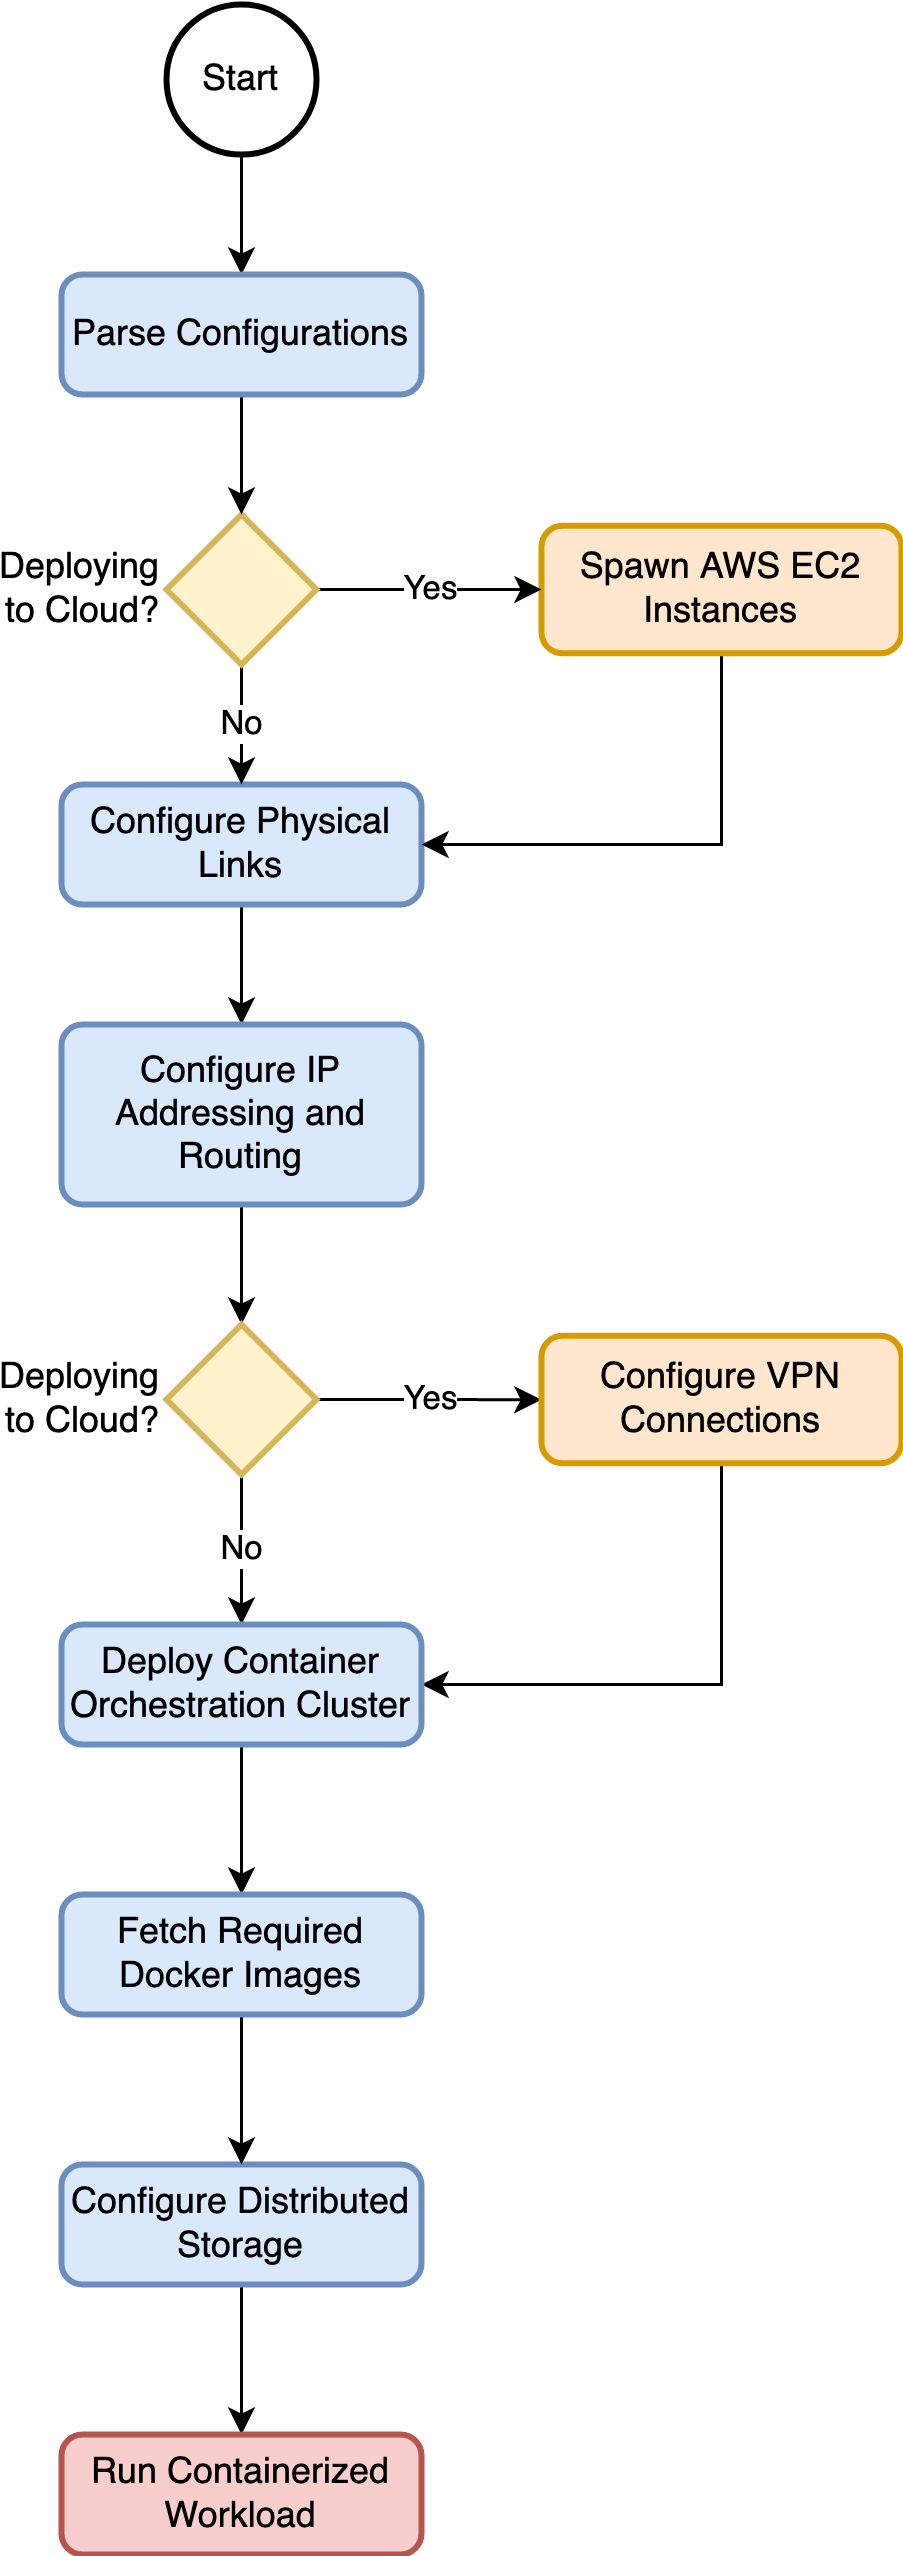
\includegraphics[width=.7\columnwidth]{figures/flow.png}
    \caption{Execution flow of Ainur.}\label{fig:flow}
\end{figure}

\Cref{fig:flow} illustrates the execution flow of Ainur.
The software follows a mostly linear approach given its direct interaction with distinct layers of hardware and networking.
Immediately after start, Ainur reads and parses the deployment configuration and parses it into a set of various dataclasses and Python dictionaries.
Next, if deploying anything to the cloud, Ainur spawns the required number of \ac{AWS} \ac{EC2} instance.
Execution then goes on to configure the physical links, connecting hosts with each other through clever management of \acp{VLAN} and \acp{SDR}.
Once physical and/or \ac{VLAN} connections are configure, \ac{IP} addresses are assigned to devices and static routes between them are configured.
If cloud instances are used, \ac{VPN} connections are established to them.
At this stage, the testbed network is fully configured, and bidirectional traffic between any two hosts is possible over the workload data network.

The next stages deal with workload deployment, scaling, and orchestration.
A \emph{Docker Swarm}\footnote{\url{https://docs.docker.com/engine/swarm/}} is deployed on the relevant hosts on the workload data network.
On top of this Swarm, required container images are fetched from a remote repository, and distributed storage is configured across all workload hosts.
Finally, the actual containerized workload is deployed as a Docker Swarm Service Stack\footnote{\url{https://docs.docker.com/engine/swarm/stack-deploy/}}, allowing us to leverage the flexibility and utilities of this orchestration platform for automatic scaling, placement, health checking, and coordination of workloads.

In terms of actual code, in practice, most steps in \cref{fig:flow} are implemented in software as abstractions of ``layers'': each step builds upon previous steps in the flow, and provides the prerequisites steps down the line expect.
Our Python implementations of these components also frequently use the \emph{context manager}\footnote{%
    For reference, see the Python documentation on \url{https://docs.python.org/3/library/contextlib.html} and associated pages.
} pattern to ensure clean teardown of the state of the testbed and the end of the execution of Ainur.
